\paragraph{Example} What is probability to get each result twice on 12 dices?
\subparagraph{Solution}
We can see the analogy - dice a ball, and result is a box, so we have 12 balls and 6 dices.


\section{Random variable}
\paragraph{Definition} $\left( \Omega, P \right)$ in called probability space.
\paragraph{Definition} Random variable $X$ on $\left( \Omega, P \right)$  is $X: \Omega \to \mathbb{R}$. We denote $\omega \in \Omega$.

$$\left\{ X  =a \right\} := \left\{ \omega \in \Omega | X(\omega) = a \right\}$$
$$\left\{a \leq  X  \leq b \right\} := \left\{ \omega \in \Omega | a\leq X(\omega) \leq b \right\}$$
$$P(X=a) := P\bigg( \left\{ X = a \right\} \bigg) = P\bigg( \left\{ \omega \in \Omega : X(\omega) = a \right\} \bigg)$$
\paragraph{Example} Two dices.
$$P\bigg((i,j)\bigg) = \frac{1}{36}$$
We can define random variable
$$X\big( (i,j) \big) = i+j$$
We can ask ourselves, what is probability that $X=7$?
$$P(X=7) = P\bigg( \left\{ (i,j) : X(i,j) = 7 \right\} \bigg) = P\bigg( \left\{ (i,j) : i+j = 7 \right\} \bigg) = \frac{1}{6}$$
\paragraph{Examples} $\Omega = [0,2]$. We can define $X(\omega) = \omega$.
$$P(0\leq X \leq 1) = P([0,1]) = \frac{1}{2}$$

\paragraph{Distribution function}
Let $X$ random variable on $(\Omega, P)$. Define $F(x) = P(X \leq x)$.
\paragraph{Example} Dices. $X=i+j$


\begin{center}
	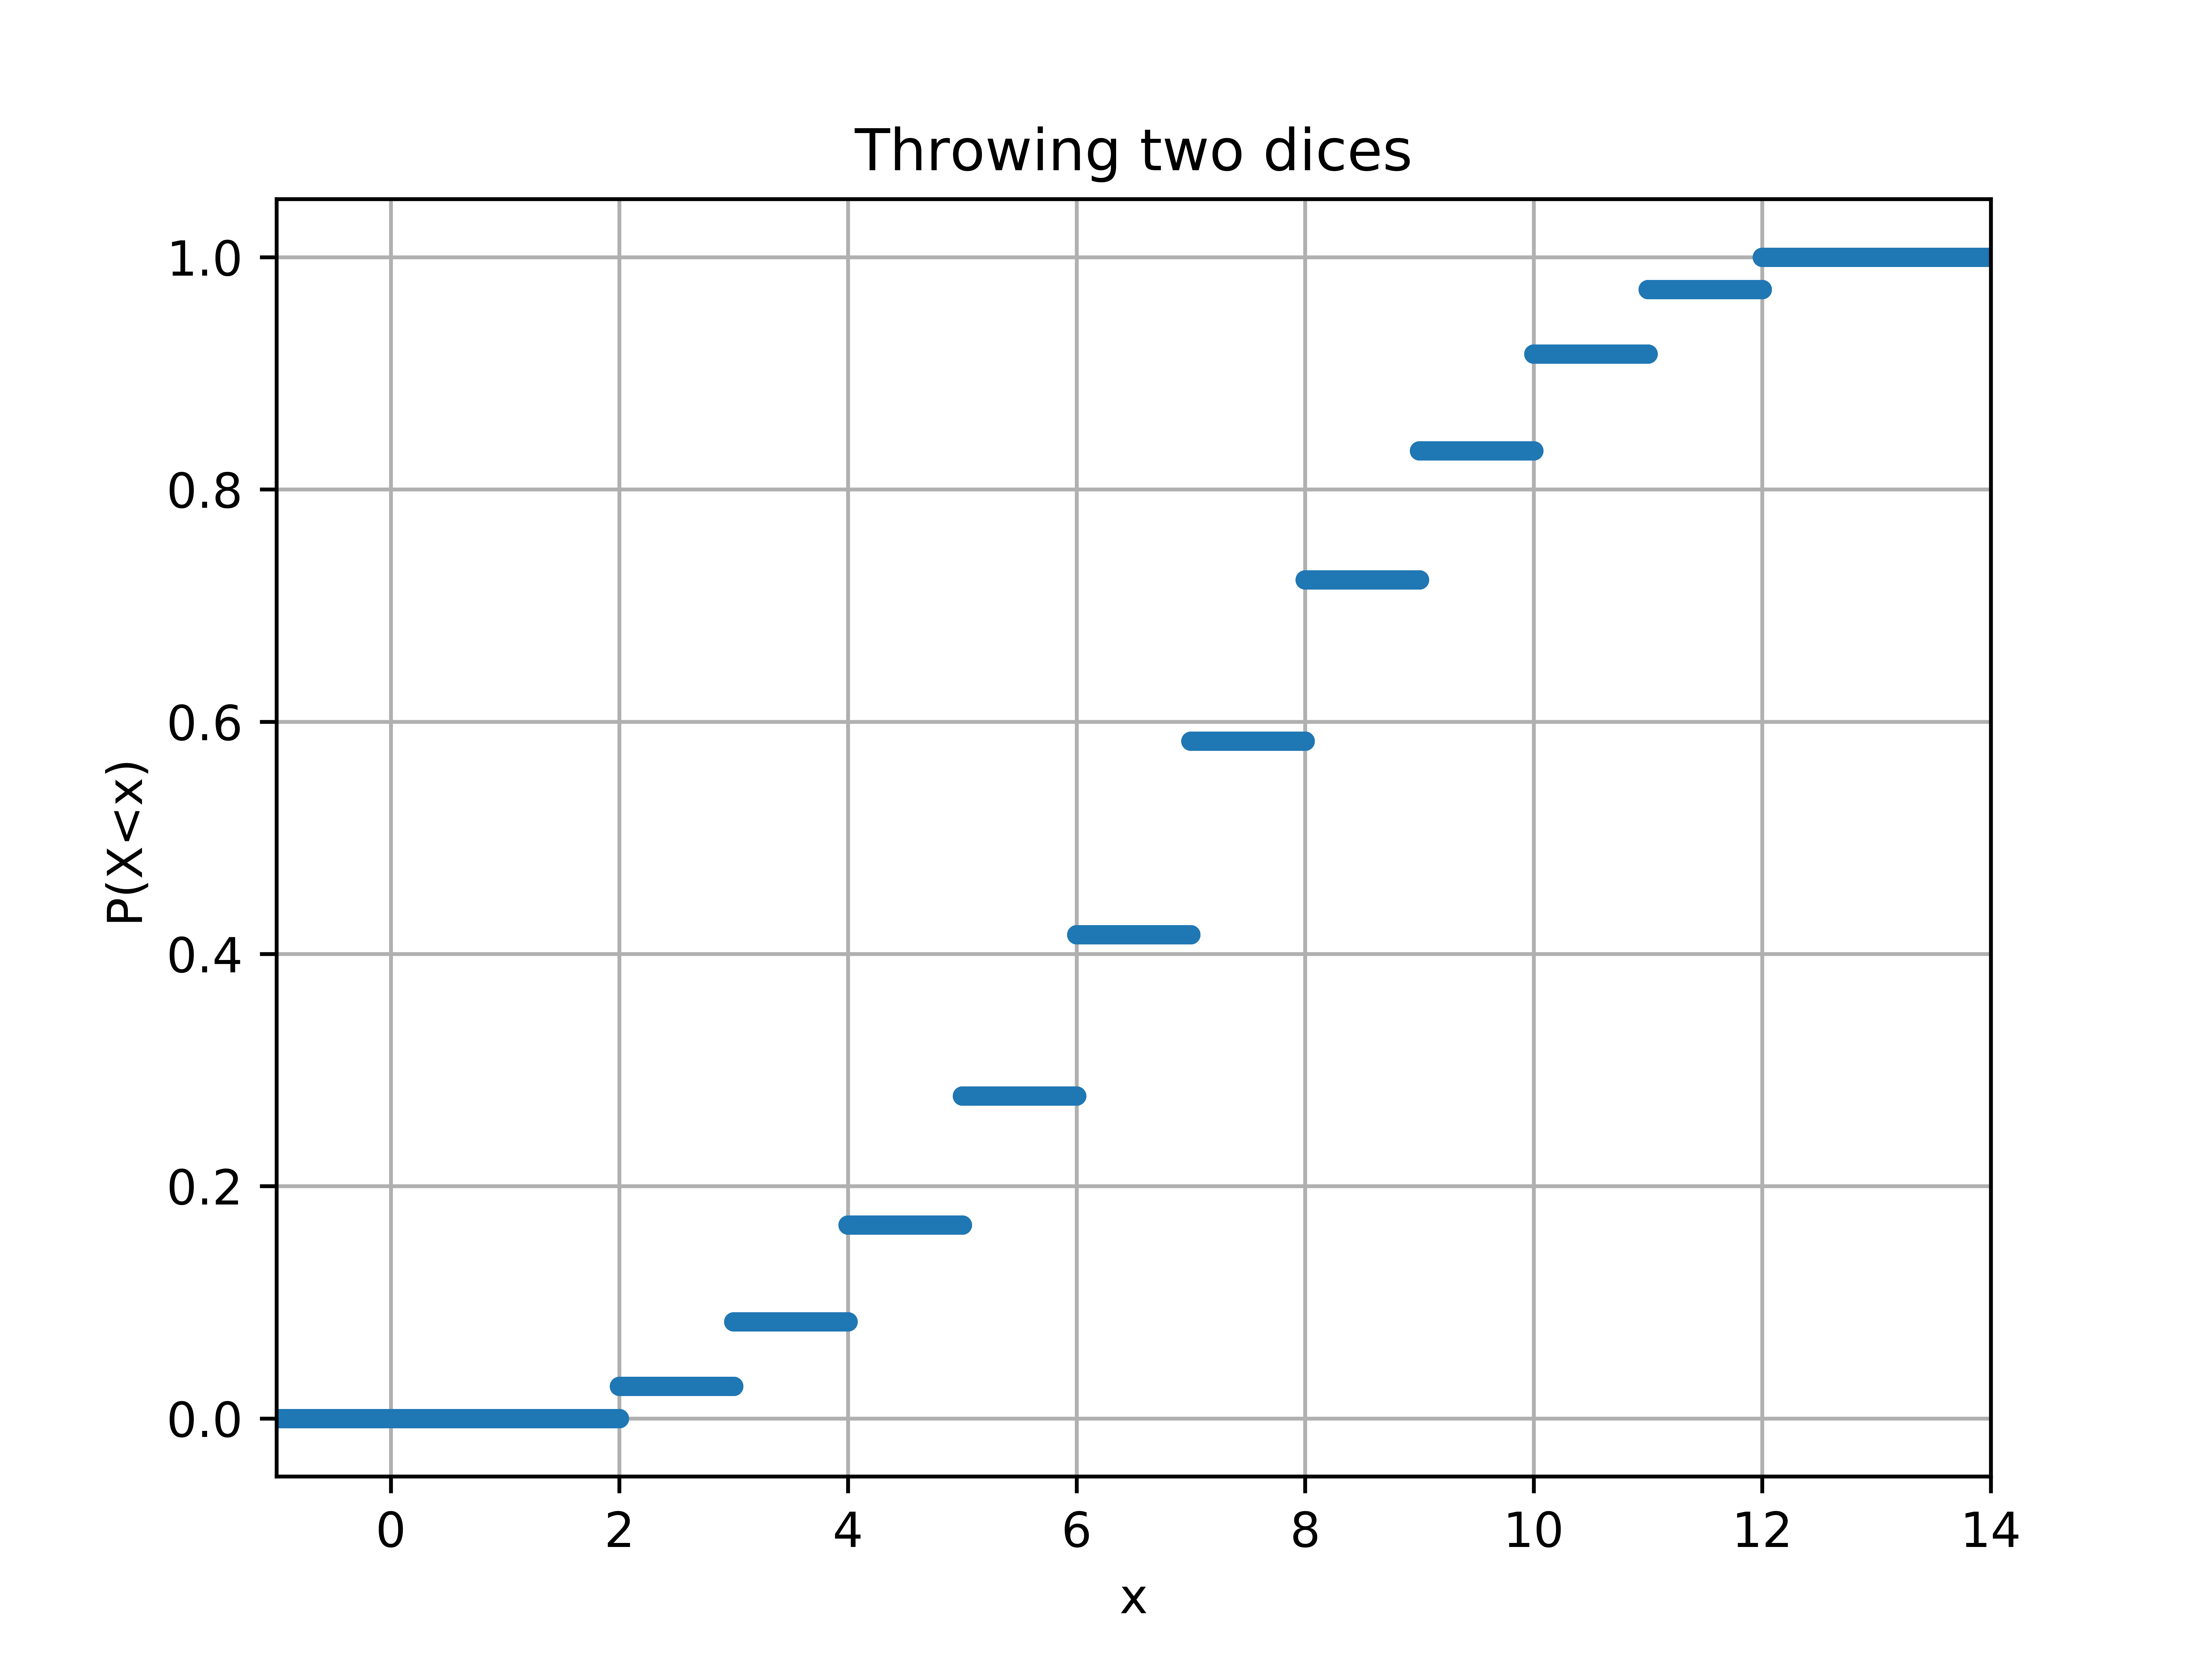
\includegraphics[width=0.5\linewidth]{./lect4/1.png}
\end{center}

\paragraph{Example} $\Omega = [0,2]$


\begin{center}
	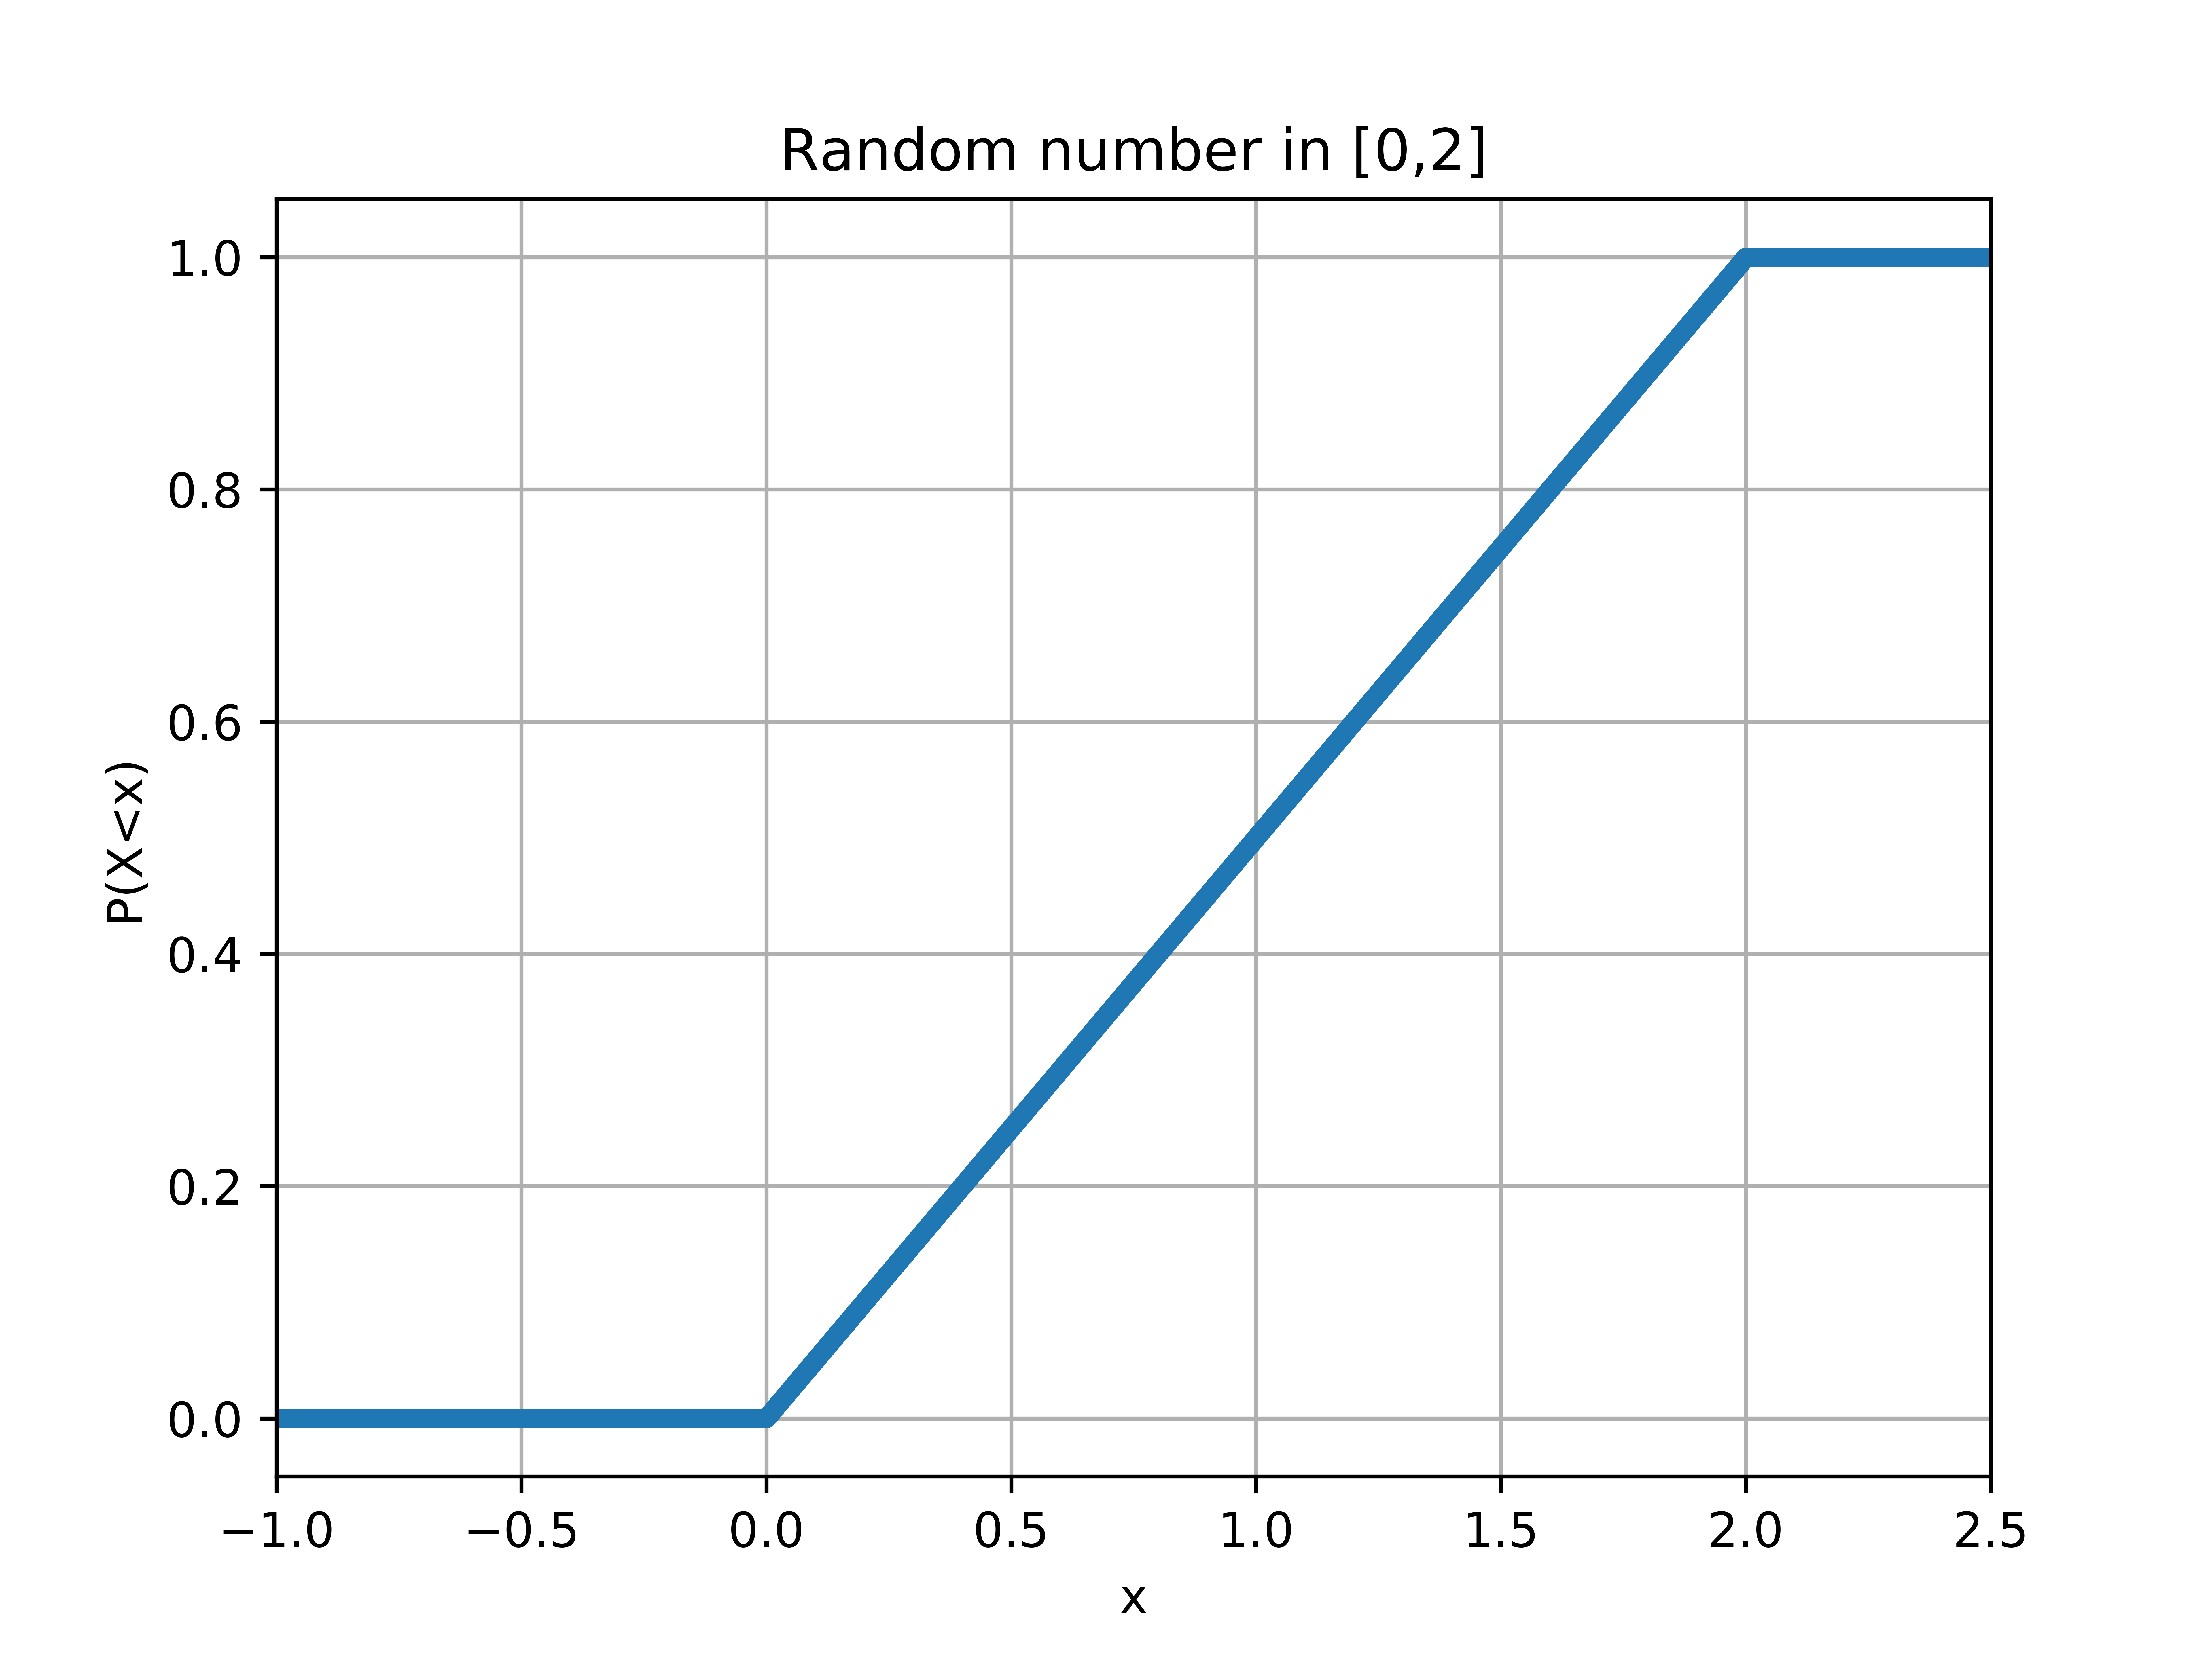
\includegraphics[width=0.5\linewidth]{./lect4/2.png}
\end{center}
